\hypertarget{FunctionDLL_8h}{
\section{/PIWO/Program/brige/FunctionDLL.h File Reference}
\label{FunctionDLL_8h}\index{/PIWO/Program/brige/FunctionDLL.h@{/PIWO/Program/brige/FunctionDLL.h}}
}
{\tt \#include $<$System.hpp$>$}\par
{\tt \#include $<$vector$>$}\par
{\tt \#include $<$exception$>$}\par
{\tt \#include $<$IniFiles.hpp$>$}\par
{\tt \#include \char`\"{}../engine/Block.h\char`\"{}}\par


Include dependency graph for FunctionDLL.h:\nopagebreak
\begin{figure}[H]
\begin{center}
\leavevmode
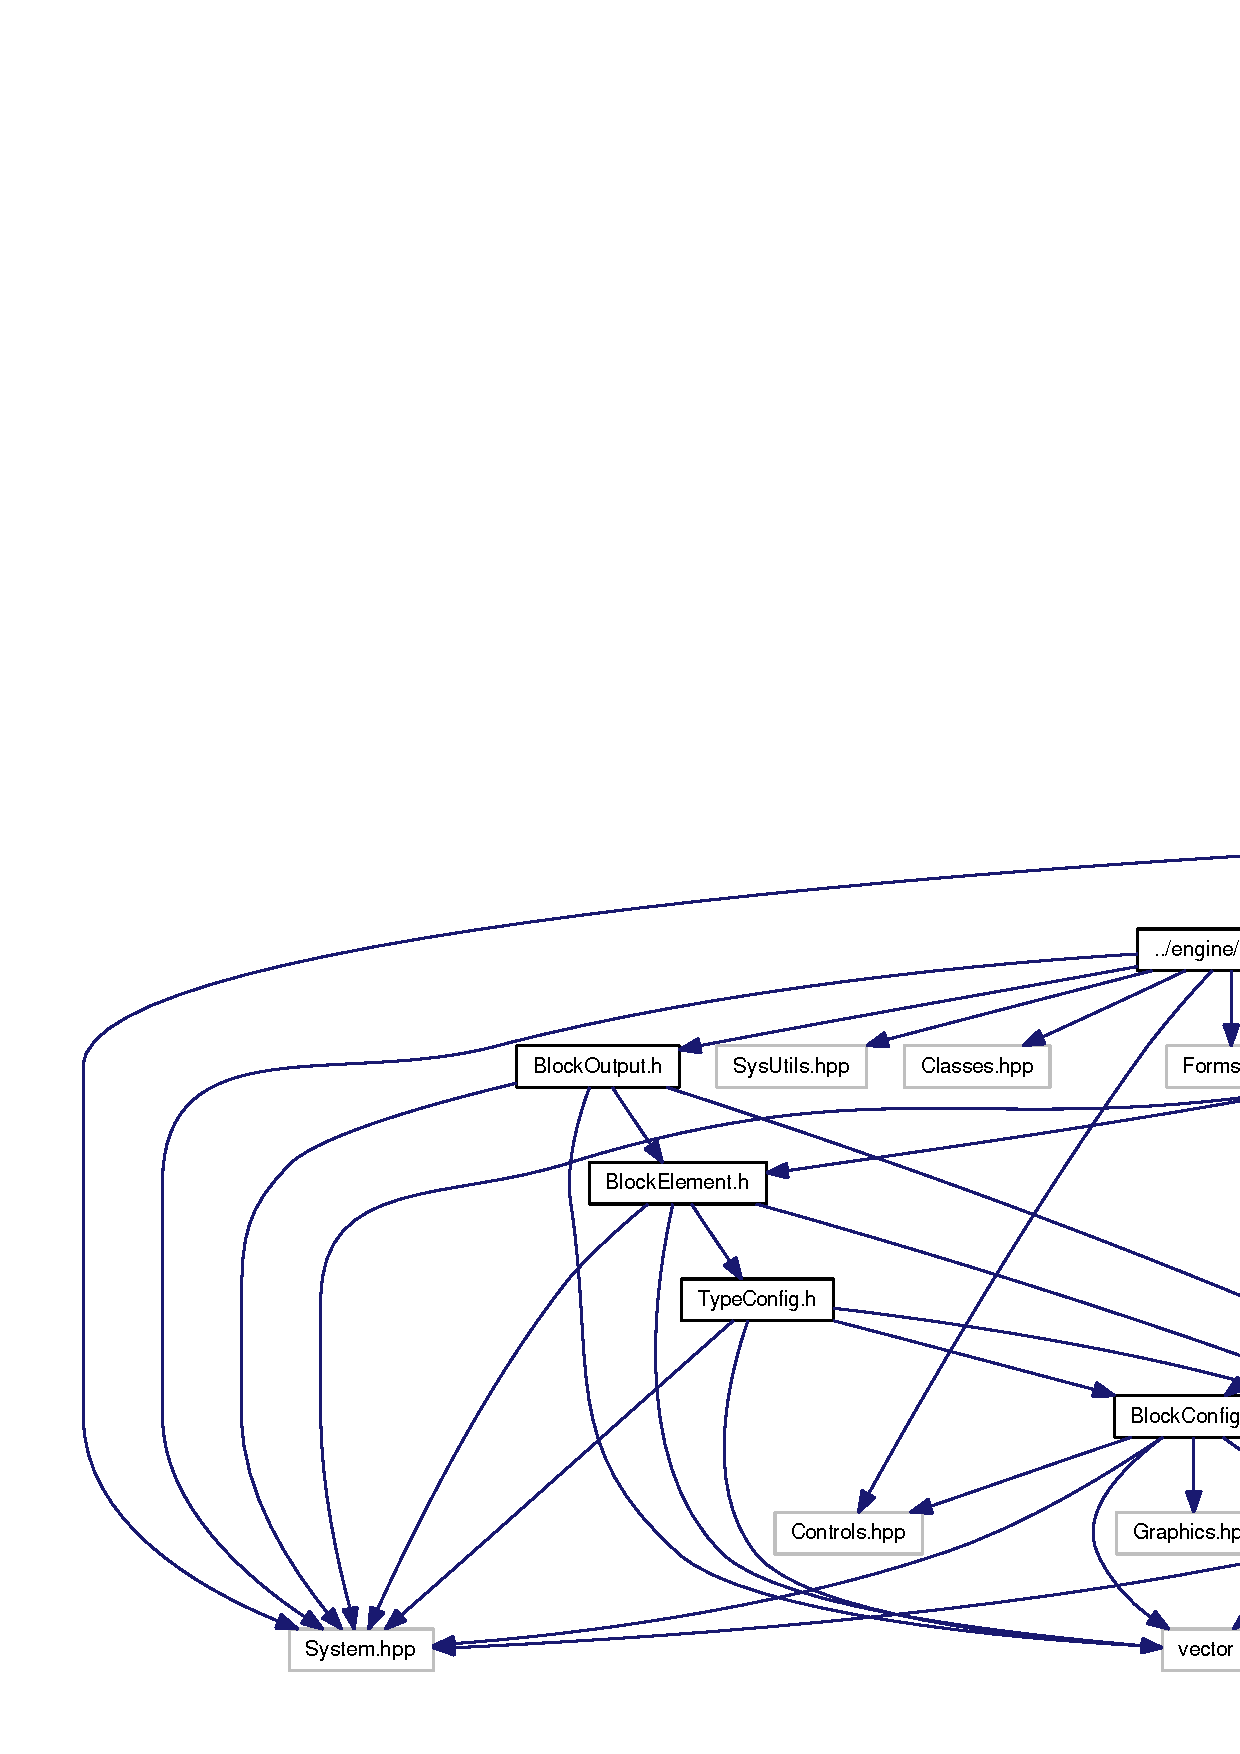
\includegraphics[width=420pt]{FunctionDLL_8h__incl}
\end{center}
\end{figure}


This graph shows which files directly or indirectly include this file:\nopagebreak
\begin{figure}[H]
\begin{center}
\leavevmode
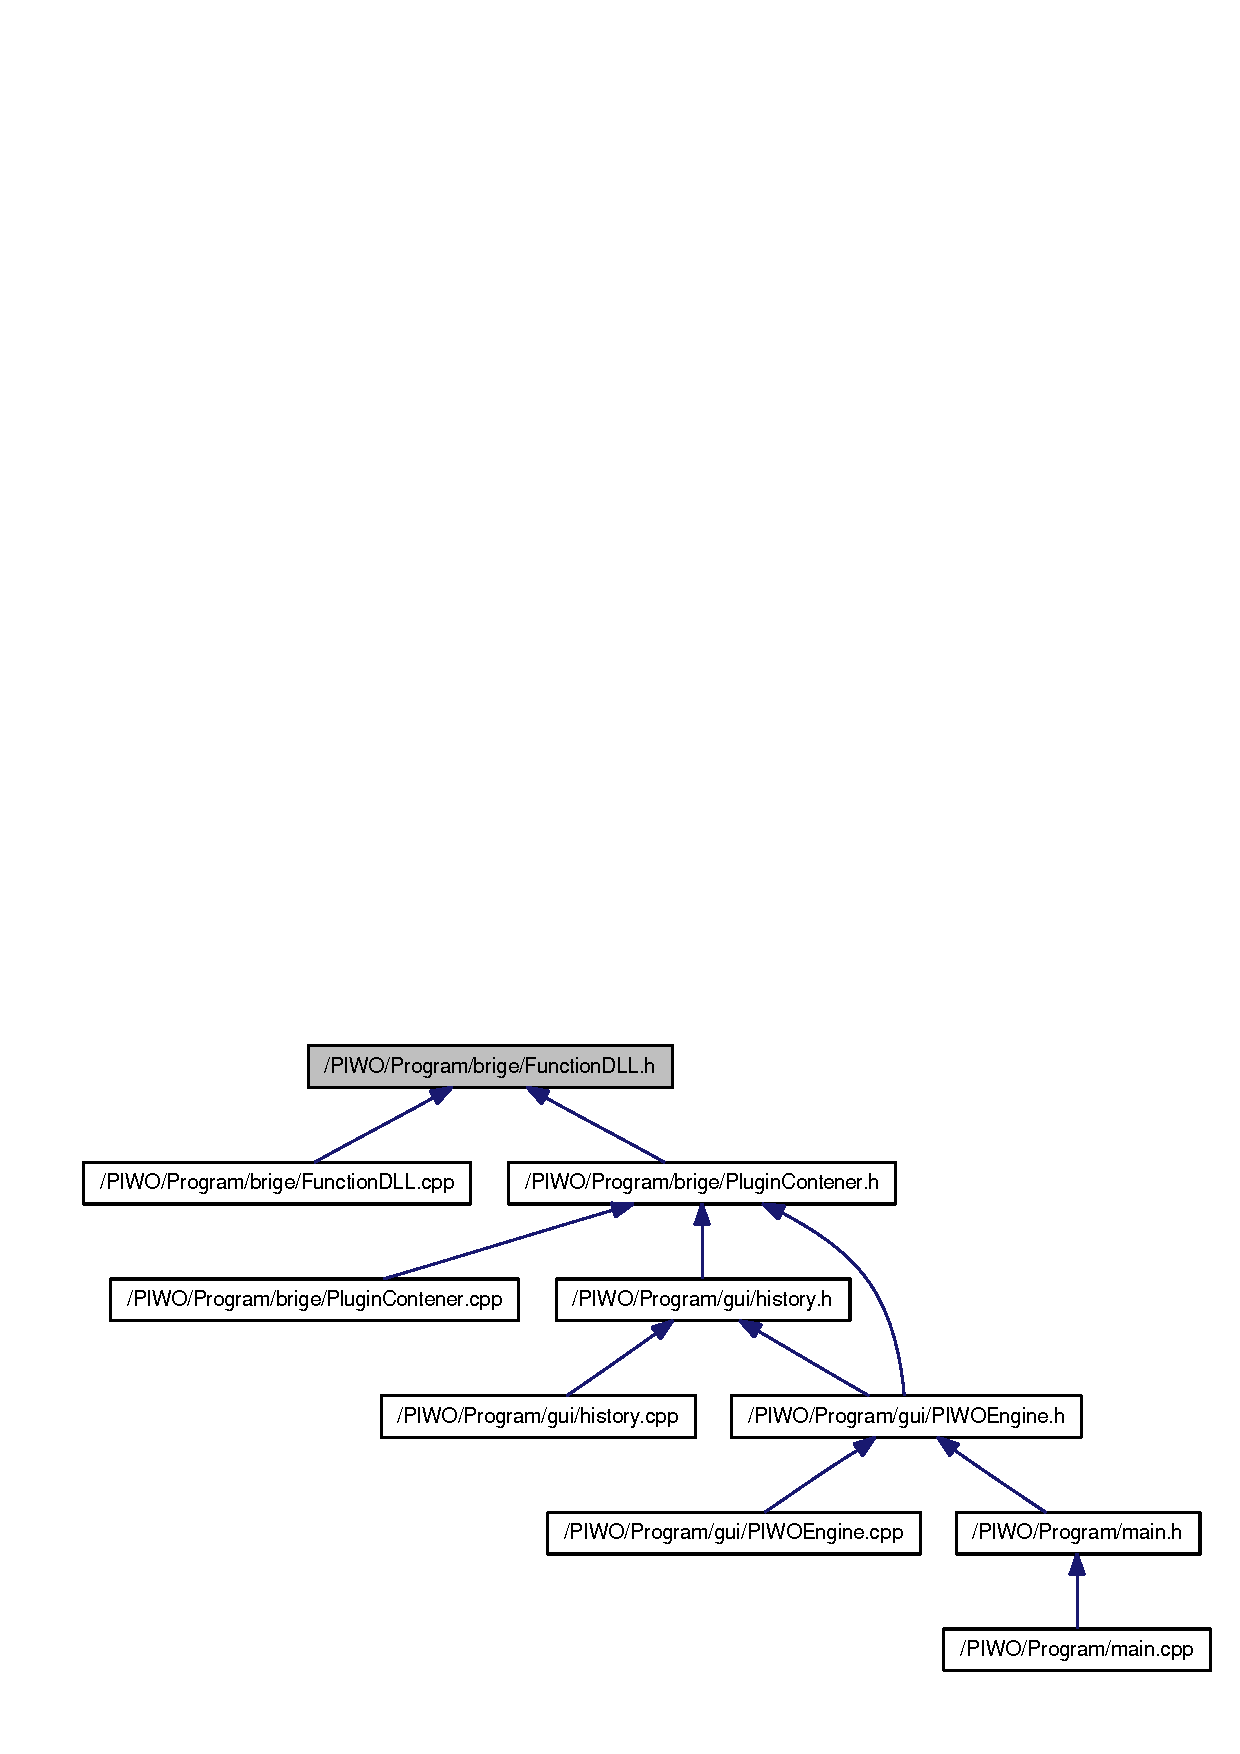
\includegraphics[width=292pt]{FunctionDLL_8h__dep__incl}
\end{center}
\end{figure}
\subsection*{Classes}
\begin{CompactItemize}
\item 
class \hyperlink{classFunctionDLL}{FunctionDLL}
\end{CompactItemize}
\subsection*{Typedefs}
\begin{CompactItemize}
\item 
typedef \hyperlink{classBlock}{Block} $\ast$typedef \hyperlink{FunctionDLL_8h_c612ada38bf83be79acb2154e3f72be6}{int} (\_\-\_\-stdcall $\ast$FunctionDLL\_\-validate)(\hyperlink{classBlock}{Block} $\ast$)
\end{CompactItemize}
\subsection*{Functions}
\begin{CompactItemize}
\item 
typedef \hyperlink{FunctionDLL_8h_2854864c4eeedd04786b0fafe1da1165}{int} (\_\-\_\-stdcall $\ast$FunctionDLL\_\-run)(\hyperlink{classBlock}{Block} $\ast$)
\item 
typedef \hyperlink{FunctionDLL_8h_9c362bc12556d578110b09d4563a7ed4}{bool} (\_\-\_\-stdcall $\ast$FunctionDLL\_\-showConfig)(TComponent $\ast$
\item 
typedef \hyperlink{FunctionDLL_8h_10f738c80bfc69a75e5d249561e4a81b}{void} (\_\-\_\-closure $\ast$FunctionDLL\_\-onClick)(void $\ast$)
\end{CompactItemize}


\subsection{Typedef Documentation}
\hypertarget{FunctionDLL_8h_c612ada38bf83be79acb2154e3f72be6}{
\index{FunctionDLL.h@{FunctionDLL.h}!int@{int}}
\index{int@{int}!FunctionDLL.h@{FunctionDLL.h}}
\subsubsection[int]{\setlength{\rightskip}{0pt plus 5cm}typedef TObject $\ast$typedef TObject $\ast$typedef TObject $\ast$typedef TObject $\ast$typedef int (\_\-\_\-stdcall $\ast$ {\em FunctionDLL\_\-validate})}}
\label{FunctionDLL_8h_c612ada38bf83be79acb2154e3f72be6}




Definition at line 14 of file FunctionDLL.h.

\subsection{Function Documentation}
\hypertarget{FunctionDLL_8h_9c362bc12556d578110b09d4563a7ed4}{
\index{FunctionDLL.h@{FunctionDLL.h}!bool@{bool}}
\index{bool@{bool}!FunctionDLL.h@{FunctionDLL.h}}
\subsubsection[bool]{\setlength{\rightskip}{0pt plus 5cm}typedef bool (\_\-\_\-stdcall $\ast$ {\em FunctionDLL\_\-showConfig})}}
\label{FunctionDLL_8h_9c362bc12556d578110b09d4563a7ed4}


\hypertarget{FunctionDLL_8h_2854864c4eeedd04786b0fafe1da1165}{
\index{FunctionDLL.h@{FunctionDLL.h}!int@{int}}
\index{int@{int}!FunctionDLL.h@{FunctionDLL.h}}
\subsubsection[int]{\setlength{\rightskip}{0pt plus 5cm}typedef int (\_\-\_\-stdcall $\ast$ {\em FunctionDLL\_\-run})}}
\label{FunctionDLL_8h_2854864c4eeedd04786b0fafe1da1165}


\hypertarget{FunctionDLL_8h_10f738c80bfc69a75e5d249561e4a81b}{
\index{FunctionDLL.h@{FunctionDLL.h}!void@{void}}
\index{void@{void}!FunctionDLL.h@{FunctionDLL.h}}
\subsubsection[void]{\setlength{\rightskip}{0pt plus 5cm}typedef TObject $\ast$typedef TObject $\ast$typedef TObject $\ast$typedef TObject $\ast$typedef void(\_\-\_\-closure $\ast$VisualBlock\_\-FunctionMove)(TObject $\ast$ (\_\-\_\-closure $\ast$ {\em FunctionDLL\_\-onClick})}}
\label{FunctionDLL_8h_10f738c80bfc69a75e5d249561e4a81b}


